\documentclass[]{article}
\usepackage{lmodern}
\usepackage{amssymb,amsmath}
\usepackage{ifxetex,ifluatex}
\usepackage{fixltx2e} % provides \textsubscript
\ifnum 0\ifxetex 1\fi\ifluatex 1\fi=0 % if pdftex
  \usepackage[T1]{fontenc}
  \usepackage[utf8]{inputenc}
\else % if luatex or xelatex
  \ifxetex
    \usepackage{mathspec}
  \else
    \usepackage{fontspec}
  \fi
  \defaultfontfeatures{Ligatures=TeX,Scale=MatchLowercase}
\fi
% use upquote if available, for straight quotes in verbatim environments
\IfFileExists{upquote.sty}{\usepackage{upquote}}{}
% use microtype if available
\IfFileExists{microtype.sty}{%
\usepackage{microtype}
\UseMicrotypeSet[protrusion]{basicmath} % disable protrusion for tt fonts
}{}
\usepackage[margin=1in]{geometry}
\usepackage{hyperref}
\hypersetup{unicode=true,
            pdftitle={Primeiro Dia - Introdução e Sintaxe},
            pdfauthor={Pedro Cavalcante},
            pdfborder={0 0 0},
            breaklinks=true}
\urlstyle{same}  % don't use monospace font for urls
\usepackage{color}
\usepackage{fancyvrb}
\newcommand{\VerbBar}{|}
\newcommand{\VERB}{\Verb[commandchars=\\\{\}]}
\DefineVerbatimEnvironment{Highlighting}{Verbatim}{commandchars=\\\{\}}
% Add ',fontsize=\small' for more characters per line
\usepackage{framed}
\definecolor{shadecolor}{RGB}{248,248,248}
\newenvironment{Shaded}{\begin{snugshade}}{\end{snugshade}}
\newcommand{\AlertTok}[1]{\textcolor[rgb]{0.94,0.16,0.16}{#1}}
\newcommand{\AnnotationTok}[1]{\textcolor[rgb]{0.56,0.35,0.01}{\textbf{\textit{#1}}}}
\newcommand{\AttributeTok}[1]{\textcolor[rgb]{0.77,0.63,0.00}{#1}}
\newcommand{\BaseNTok}[1]{\textcolor[rgb]{0.00,0.00,0.81}{#1}}
\newcommand{\BuiltInTok}[1]{#1}
\newcommand{\CharTok}[1]{\textcolor[rgb]{0.31,0.60,0.02}{#1}}
\newcommand{\CommentTok}[1]{\textcolor[rgb]{0.56,0.35,0.01}{\textit{#1}}}
\newcommand{\CommentVarTok}[1]{\textcolor[rgb]{0.56,0.35,0.01}{\textbf{\textit{#1}}}}
\newcommand{\ConstantTok}[1]{\textcolor[rgb]{0.00,0.00,0.00}{#1}}
\newcommand{\ControlFlowTok}[1]{\textcolor[rgb]{0.13,0.29,0.53}{\textbf{#1}}}
\newcommand{\DataTypeTok}[1]{\textcolor[rgb]{0.13,0.29,0.53}{#1}}
\newcommand{\DecValTok}[1]{\textcolor[rgb]{0.00,0.00,0.81}{#1}}
\newcommand{\DocumentationTok}[1]{\textcolor[rgb]{0.56,0.35,0.01}{\textbf{\textit{#1}}}}
\newcommand{\ErrorTok}[1]{\textcolor[rgb]{0.64,0.00,0.00}{\textbf{#1}}}
\newcommand{\ExtensionTok}[1]{#1}
\newcommand{\FloatTok}[1]{\textcolor[rgb]{0.00,0.00,0.81}{#1}}
\newcommand{\FunctionTok}[1]{\textcolor[rgb]{0.00,0.00,0.00}{#1}}
\newcommand{\ImportTok}[1]{#1}
\newcommand{\InformationTok}[1]{\textcolor[rgb]{0.56,0.35,0.01}{\textbf{\textit{#1}}}}
\newcommand{\KeywordTok}[1]{\textcolor[rgb]{0.13,0.29,0.53}{\textbf{#1}}}
\newcommand{\NormalTok}[1]{#1}
\newcommand{\OperatorTok}[1]{\textcolor[rgb]{0.81,0.36,0.00}{\textbf{#1}}}
\newcommand{\OtherTok}[1]{\textcolor[rgb]{0.56,0.35,0.01}{#1}}
\newcommand{\PreprocessorTok}[1]{\textcolor[rgb]{0.56,0.35,0.01}{\textit{#1}}}
\newcommand{\RegionMarkerTok}[1]{#1}
\newcommand{\SpecialCharTok}[1]{\textcolor[rgb]{0.00,0.00,0.00}{#1}}
\newcommand{\SpecialStringTok}[1]{\textcolor[rgb]{0.31,0.60,0.02}{#1}}
\newcommand{\StringTok}[1]{\textcolor[rgb]{0.31,0.60,0.02}{#1}}
\newcommand{\VariableTok}[1]{\textcolor[rgb]{0.00,0.00,0.00}{#1}}
\newcommand{\VerbatimStringTok}[1]{\textcolor[rgb]{0.31,0.60,0.02}{#1}}
\newcommand{\WarningTok}[1]{\textcolor[rgb]{0.56,0.35,0.01}{\textbf{\textit{#1}}}}
\usepackage{graphicx,grffile}
\makeatletter
\def\maxwidth{\ifdim\Gin@nat@width>\linewidth\linewidth\else\Gin@nat@width\fi}
\def\maxheight{\ifdim\Gin@nat@height>\textheight\textheight\else\Gin@nat@height\fi}
\makeatother
% Scale images if necessary, so that they will not overflow the page
% margins by default, and it is still possible to overwrite the defaults
% using explicit options in \includegraphics[width, height, ...]{}
\setkeys{Gin}{width=\maxwidth,height=\maxheight,keepaspectratio}
\IfFileExists{parskip.sty}{%
\usepackage{parskip}
}{% else
\setlength{\parindent}{0pt}
\setlength{\parskip}{6pt plus 2pt minus 1pt}
}
\setlength{\emergencystretch}{3em}  % prevent overfull lines
\providecommand{\tightlist}{%
  \setlength{\itemsep}{0pt}\setlength{\parskip}{0pt}}
\setcounter{secnumdepth}{0}
% Redefines (sub)paragraphs to behave more like sections
\ifx\paragraph\undefined\else
\let\oldparagraph\paragraph
\renewcommand{\paragraph}[1]{\oldparagraph{#1}\mbox{}}
\fi
\ifx\subparagraph\undefined\else
\let\oldsubparagraph\subparagraph
\renewcommand{\subparagraph}[1]{\oldsubparagraph{#1}\mbox{}}
\fi

%%% Use protect on footnotes to avoid problems with footnotes in titles
\let\rmarkdownfootnote\footnote%
\def\footnote{\protect\rmarkdownfootnote}

%%% Change title format to be more compact
\usepackage{titling}

% Create subtitle command for use in maketitle
\providecommand{\subtitle}[1]{
  \posttitle{
    \begin{center}\large#1\end{center}
    }
}

\setlength{\droptitle}{-2em}

  \title{Primeiro Dia - Introdução e Sintaxe}
    \pretitle{\vspace{\droptitle}\centering\huge}
  \posttitle{\par}
    \author{Pedro Cavalcante}
    \preauthor{\centering\large\emph}
  \postauthor{\par}
      \predate{\centering\large\emph}
  \postdate{\par}
    \date{20 de fevereiro de 2019}


\begin{document}
\maketitle

\hypertarget{o-que-e-r}{%
\section{O que é R}\label{o-que-e-r}}

R é uma linguagem de programação voltada para estatística e análise de
dados \emph{open-source}, gratuita e de natureza colaborativa. Como
vamos ver, o ambiente voltado para análise de dados facilita enormemente
as tarefas do ciclo.

\begin{figure}
\centering
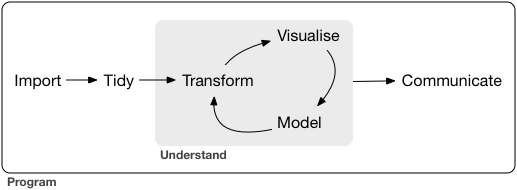
\includegraphics{https://d33wubrfki0l68.cloudfront.net/571b056757d68e6df81a3e3853f54d3c76ad6efc/32d37/diagrams/data-science.png}
\caption{O ciclo da análise de dados}
\end{figure}

Instalar o R é muito simples, ele está disponível em
\url{http://cran.r-project.org/}. É importante depois instalar o
RStudio, disponível em \url{https://www.rstudio.org/}, que é uma IDE
(Integrated Development Enviroment). IDEs são progrmas que facilitam, e
muito, programar porque trazem um ambiente gráfico mais intuitivo,
disponibilizando informações como quais objetos estão carregados na
memória do computador, visualização de gráficos e animações que fazemos
e por aí vai.

\begin{figure}
\centering
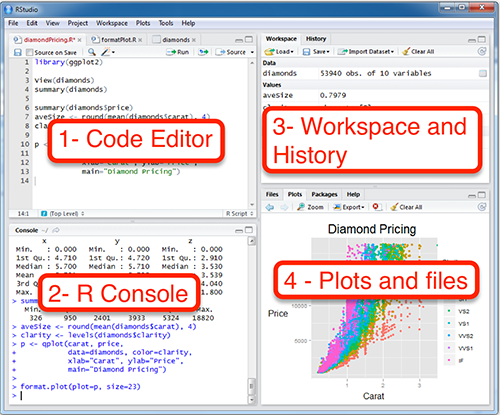
\includegraphics{http://www.sthda.com/sthda/RDoc/images/rstudio.png}
\caption{O ambiente do RStudio}
\end{figure}

\hypertarget{links-importantes}{%
\section{Links importantes}\label{links-importantes}}

\begin{itemize}
\tightlist
\item
  \href{https://github.com}{Github}
\end{itemize}

É como uma ``rede social de códigos'' com várias funcionalidades úteis
para cuidar dos seus códigos e gerenciar projetos. É muito importante
fazer uma conta lá e usar o programa para lidar adequadamente com o
armazenamento dos códigos. O Github é particularmente útil para
trabalhar com outras pessoas porque armazena versões antigas, quem fez
que alterações nos códigos, evita conflito entre versões de programas e
mantém tudo numa fonte única e facilmente acessível.

\begin{itemize}
\tightlist
\item
  \href{https://stackoverflow.com/}{StackOverflow}
\end{itemize}

Um fórum extremamente popular em inglês sobre programação. A maior parte
das suas dúvidas já foi resolvida lá e se não foi, é muito simples fazer
uma nova pergunta.

\begin{itemize}
\tightlist
\item
  \href{https://stats.stackexchange.com/}{CrossValidated}
\end{itemize}

Uma espécie de StackOverflow, mas voltada para análise de dados. Quando
a dúvida for mais estatístisca do que de programação em si, é melhor
conferir aqui. A maioria dos usuários sabe R e vai pedir algum pedaço de
código para entender o seu problema bem.

\begin{itemize}
\tightlist
\item
  \href{https://danmrc.github.io/R-para-Economistas/}{R: Uma Introdução
  para Economistas}
\end{itemize}

Uma fonte ótima para consultas rápidas.

\begin{itemize}
\tightlist
\item
  \href{https://r4ds.had.co.nz}{R for Data Science}
\end{itemize}

A fonte definitiva do R introdutório. É um livro em inglês muito extenso
e deve cobrir razoavelmente qualquer assunto que um iniciante queira
entender melhor.

\hypertarget{os-primeiros-comandos}{%
\section{Os primeiros comandos}\label{os-primeiros-comandos}}

Tenha em mente que você pode anotar linhas de código na área do script e
rodar linhas específicas copiando-as no console, digiando-as diretamente
lá ou selecionando o trecho do script desejado e apertando
\texttt{ctrl\ +\ enter}.

A grande vantagem do R é sua naturza colaborativa. Pesquisadores,
programadores, profissionais e entusiastas do mundo todo escrevem
\emph{pacotes} com funcionalidades novas, que incluem coisas como
ferramentas para econometria bayseana, gerar animaçãoes, estimar
dinâmicas evolutivas, resolver problemas de otimização e gerir blogs.
Pacotes tem nomes e eles trazem \emph{funções} novas. Normalmente nos
referimos a uma função na forma \texttt{pacote::função} ou
\texttt{função()}. Então se lemos \texttt{dplyr::filter} sabemos que é a
função \texttt{filter()} do pacote \texttt{dplyr}.

Alguns pacotes já vêm carregados no R, eles são o que chamamos de
Biblioteca Padrão, a versão mais simples do R. Os mais importantes
pacotes da BP são o \texttt{base} com toda a sintaxe básica da
linguagem, o \texttt{stats} com dezenas de ferramentas estatísticas
muito úteis e o \texttt{utils} com várias funções miscelâneas.

No entanto, a maioria dos pacotes não vem carregada no R diretamente.
Eles estão sediados no que chamamos de Comprehensive R Archive Network
(CRAN). Podemos instalar esses pacotes facilmente e depois é simples
carrega-los. Vamos baixar o \texttt{rootSolve}, que traz funções para
resolver equações e problemas de cálculo diferencial.

\begin{Shaded}
\begin{Highlighting}[]
\KeywordTok{install.packages}\NormalTok{(}\StringTok{"rootSolve"}\NormalTok{)}
\KeywordTok{library}\NormalTok{(rootSolve)}
\end{Highlighting}
\end{Shaded}

\texttt{install.packages()} só precisa que você dê o nome do pacote que
o R instala para você. \texttt{library()} serve para carregar o pacote e
ter essas funções novas disponíveis. Para saber quem fez o pacote e como
devemos cita-lo em trabalhos acadêmicos, basta usar \texttt{citation()}.

\begin{Shaded}
\begin{Highlighting}[]
\KeywordTok{citation}\NormalTok{(}\StringTok{"rootSolve"}\NormalTok{)}
\end{Highlighting}
\end{Shaded}

\begin{verbatim}
## 
## To cite package 'rootSolve' in publications use:
## 
##   Soetaert K. and P.M.J. Herman (2009).  A Practical Guide to
##   Ecological Modelling. Using R as a Simulation Platform.
##   Springer, 372 pp.
## 
##   Soetaert K. (2009).  rootSolve: Nonlinear root finding,
##   equilibrium and steady-state analysis of ordinary differential
##   equations.  R-package version 1.6
## 
## rootSolve was created to solve the examples from chapter 7 of our
## book - please cite this book when using it, thank you!
## To see these entries in BibTeX format, use 'print(<citation>,
## bibtex=TRUE)', 'toBibtex(.)', or set
## 'options(citation.bibtex.max=999)'.
\end{verbatim}

Agora vamos cobrir alguns aspectos básicos da sintaxe do R.

\hypertarget{uma-calculadora-potente}{%
\section{Uma calculadora potente}\label{uma-calculadora-potente}}

A maneira mais simples de pensar no R é como uma calculadora. Observe
que podemos usar \texttt{\#} para fazer comentários no código, isso é
útil para deixar tudo mais legível.

\begin{Shaded}
\begin{Highlighting}[]
\DecValTok{2} \OperatorTok{+}\StringTok{ }\DecValTok{2} \CommentTok{# soma simples}
\end{Highlighting}
\end{Shaded}

\begin{verbatim}
## [1] 4
\end{verbatim}

\begin{Shaded}
\begin{Highlighting}[]
\DecValTok{2} \OperatorTok{-}\StringTok{ }\DecValTok{1} \CommentTok{# subtração}
\end{Highlighting}
\end{Shaded}

\begin{verbatim}
## [1] 1
\end{verbatim}

\begin{Shaded}
\begin{Highlighting}[]
\DecValTok{2}\OperatorTok{^}\DecValTok{3} \CommentTok{# elevar ao cubo}
\end{Highlighting}
\end{Shaded}

\begin{verbatim}
## [1] 8
\end{verbatim}

\begin{Shaded}
\begin{Highlighting}[]
\DecValTok{2}\OperatorTok{*}\DecValTok{3} \CommentTok{#multiplicação}
\end{Highlighting}
\end{Shaded}

\begin{verbatim}
## [1] 6
\end{verbatim}

\begin{Shaded}
\begin{Highlighting}[]
\DecValTok{-2}\OperatorTok{*}\DecValTok{3} \CommentTok{# multiplicação por um negativo}
\end{Highlighting}
\end{Shaded}

\begin{verbatim}
## [1] -6
\end{verbatim}

\begin{Shaded}
\begin{Highlighting}[]
\DecValTok{2}\OperatorTok{**}\DecValTok{3} \CommentTok{# forma alternativa de elevar à potências}
\end{Highlighting}
\end{Shaded}

\begin{verbatim}
## [1] 8
\end{verbatim}

Também podemos fazer testes lógicos usando o \texttt{==} para igual ou
\texttt{!=} para diferente.

\begin{Shaded}
\begin{Highlighting}[]
\DecValTok{2} \OperatorTok{+}\StringTok{ }\DecValTok{2} \OperatorTok{==}\StringTok{ }\DecValTok{4} \CommentTok{# testando se 2 + 2 = 4}
\end{Highlighting}
\end{Shaded}

\begin{verbatim}
## [1] TRUE
\end{verbatim}

\begin{Shaded}
\begin{Highlighting}[]
\DecValTok{2} \OperatorTok{+}\StringTok{ }\DecValTok{2} \OperatorTok{!=}\StringTok{ }\DecValTok{4} \CommentTok{# agora se é diferente}
\end{Highlighting}
\end{Shaded}

\begin{verbatim}
## [1] FALSE
\end{verbatim}

\begin{Shaded}
\begin{Highlighting}[]
\DecValTok{2} \OperatorTok{+}\StringTok{ }\DecValTok{2} \OperatorTok{>}\StringTok{ }\DecValTok{3} \CommentTok{# maior}
\end{Highlighting}
\end{Shaded}

\begin{verbatim}
## [1] TRUE
\end{verbatim}

\begin{Shaded}
\begin{Highlighting}[]
\DecValTok{2} \OperatorTok{+}\StringTok{ }\DecValTok{2} \OperatorTok{<}\StringTok{ }\DecValTok{3} \CommentTok{# menor}
\end{Highlighting}
\end{Shaded}

\begin{verbatim}
## [1] FALSE
\end{verbatim}

\begin{Shaded}
\begin{Highlighting}[]
\OtherTok{TRUE} \OperatorTok{==}\StringTok{ }\OtherTok{FALSE} \CommentTok{# podemos também testar proposições lógicas mais abstratas}
\end{Highlighting}
\end{Shaded}

\begin{verbatim}
## [1] FALSE
\end{verbatim}

No entanto, a maior parte do tempo lidaremos com \emph{objetos}, que
iremos definir com o sinal \texttt{\textless{}-}, que chamamos de
Operador de Designação (Assignment Operator). Se parecer muito estranho
digitar isso, o atalho é \texttt{Alt} + \texttt{-}. Você também pode
usar o sinal \texttt{=}, ele vai funcionar quase sempre como um
sinônimo, mas talvez possa te confundir se estiver fazendo testes
lógicos, então use com cuidado.

\begin{Shaded}
\begin{Highlighting}[]
\NormalTok{a =}\StringTok{ }\DecValTok{2} \CommentTok{# definindo um objeto a como 2}
\NormalTok{b <-}\StringTok{ }\DecValTok{2} \CommentTok{# o mesmo com b, usando o sinal <-}

\NormalTok{a }\OperatorTok{==}\StringTok{ }\NormalTok{b }\CommentTok{# teste lógico}
\end{Highlighting}
\end{Shaded}

\begin{verbatim}
## [1] TRUE
\end{verbatim}

Temos também como usar funções, pedaços prontos de código com
funcionalidades específicas. Funções podem ou não admitir
\emph{argumentos}, que são especificados usando seu nome, um sinal de
\texttt{=} e o valor do argumento, todos separados por vírgula. Por
questões de organização de código, é bom pular uma linha para cada
argumento, embora você possa usar formas alternativas de identação.
Algumas funções são simples o suficiente para que você não precisa dizer
exatamente qual argumento é qual, como é o caso de \texttt{seq()}.
\texttt{seq()} também tem outra pecualiaridade, seu argumento
\texttt{by}, que informa o tamanho do passo entre um elemento e outro da
sequência é por padrão o número 1. Descobrimos isso lendo a documentação
da função. Você pode acessa-la pela função \texttt{help()} ou apertando
\texttt{F1} quando o cursor estiver em cima da funçaõ.

\begin{Shaded}
\begin{Highlighting}[]
\KeywordTok{help}\NormalTok{(seq)}
\end{Highlighting}
\end{Shaded}

\begin{Shaded}
\begin{Highlighting}[]
\KeywordTok{print}\NormalTok{(a) }\CommentTok{# retorna no console o valor de a}
\end{Highlighting}
\end{Shaded}

\begin{verbatim}
## [1] 2
\end{verbatim}

\begin{Shaded}
\begin{Highlighting}[]
\KeywordTok{exp}\NormalTok{(}\DecValTok{4}\NormalTok{) }\CommentTok{# exponencial}
\end{Highlighting}
\end{Shaded}

\begin{verbatim}
## [1] 54.59815
\end{verbatim}

\begin{Shaded}
\begin{Highlighting}[]
\KeywordTok{factorial}\NormalTok{(}\DecValTok{4}\NormalTok{) }\CommentTok{# fatorial}
\end{Highlighting}
\end{Shaded}

\begin{verbatim}
## [1] 24
\end{verbatim}

\begin{Shaded}
\begin{Highlighting}[]
\KeywordTok{sqrt}\NormalTok{(}\DecValTok{9}\NormalTok{) }\CommentTok{# raiz quadrada}
\end{Highlighting}
\end{Shaded}

\begin{verbatim}
## [1] 3
\end{verbatim}

\begin{Shaded}
\begin{Highlighting}[]
\KeywordTok{choose}\NormalTok{(}\DecValTok{4}\NormalTok{, }\DecValTok{2}\NormalTok{) }\CommentTok{# permutação de 4, 2 a 2}
\end{Highlighting}
\end{Shaded}

\begin{verbatim}
## [1] 6
\end{verbatim}

\begin{Shaded}
\begin{Highlighting}[]
\KeywordTok{seq}\NormalTok{(}\DataTypeTok{from =} \DecValTok{1}\NormalTok{,}
    \DataTypeTok{to =} \DecValTok{10}\NormalTok{, }
    \DataTypeTok{by =} \DecValTok{2}\NormalTok{) }\CommentTok{#sequência de-para com passo 2}
\end{Highlighting}
\end{Shaded}

\begin{verbatim}
## [1] 1 3 5 7 9
\end{verbatim}

\begin{Shaded}
\begin{Highlighting}[]
\KeywordTok{seq}\NormalTok{(}\DecValTok{1}\NormalTok{, }\DecValTok{10}\NormalTok{, }\DecValTok{2}\NormalTok{) }\CommentTok{# o mesmo resultado sem especificar qual argumento é qual}
\end{Highlighting}
\end{Shaded}

\begin{verbatim}
## [1] 1 3 5 7 9
\end{verbatim}

\begin{Shaded}
\begin{Highlighting}[]
\NormalTok{c =}\StringTok{ }\KeywordTok{seq}\NormalTok{(}\DecValTok{1}\NormalTok{, }\DecValTok{5}\NormalTok{, }\DecValTok{1}\NormalTok{) }\CommentTok{# agora com um passo 1}

\DecValTok{1}\OperatorTok{:}\DecValTok{5} \CommentTok{# usar : também serve para gerar sequências com passo 1}
\end{Highlighting}
\end{Shaded}

\begin{verbatim}
## [1] 1 2 3 4 5
\end{verbatim}

\begin{Shaded}
\begin{Highlighting}[]
\KeywordTok{print}\NormalTok{(c)}
\end{Highlighting}
\end{Shaded}

\begin{verbatim}
## [1] 1 2 3 4 5
\end{verbatim}

\begin{Shaded}
\begin{Highlighting}[]
\KeywordTok{sum}\NormalTok{(c) }\CommentTok{# soma das entradas}
\end{Highlighting}
\end{Shaded}

\begin{verbatim}
## [1] 15
\end{verbatim}

Observe que o objeto \texttt{c} é um pouco diferente dos anteriores, que
eram só um número. \texttt{c} tem uma sequência. Para descobrir a classe
de um objeto, usamos a função \texttt{class()} e para inspeciona-lo
melhor usar \texttt{str()} (uma abreviação de estrutura em inglês).

\begin{Shaded}
\begin{Highlighting}[]
\KeywordTok{class}\NormalTok{(a)}
\end{Highlighting}
\end{Shaded}

\begin{verbatim}
## [1] "numeric"
\end{verbatim}

\begin{Shaded}
\begin{Highlighting}[]
\KeywordTok{str}\NormalTok{(a)}
\end{Highlighting}
\end{Shaded}

\begin{verbatim}
##  num 2
\end{verbatim}

\begin{Shaded}
\begin{Highlighting}[]
\KeywordTok{class}\NormalTok{(c)}
\end{Highlighting}
\end{Shaded}

\begin{verbatim}
## [1] "numeric"
\end{verbatim}

\begin{Shaded}
\begin{Highlighting}[]
\KeywordTok{str}\NormalTok{(c)}
\end{Highlighting}
\end{Shaded}

\begin{verbatim}
##  num [1:5] 1 2 3 4 5
\end{verbatim}

Uma das estruturas de dados mais importantes do R são vetores. Podemos
declarar vetores de várias formas, uma ``simples'' é usando a função
\texttt{c()}. Para saber se um objeto é vetor, podemos usar
\texttt{is.vector()}. Objetos podem ser nomeados com números, desde que
não comecem com um número. Letras maísculas e minúsculas também fazem
diferença.

\begin{Shaded}
\begin{Highlighting}[]
\NormalTok{A =}\StringTok{ }\KeywordTok{c}\NormalTok{(}\DecValTok{2}\NormalTok{,}\DecValTok{2}\NormalTok{) }\CommentTok{# A é um vetor de duas dimensões em que cada entrada é um 2}

\KeywordTok{print}\NormalTok{(A) }\CommentTok{# printamos no console}
\end{Highlighting}
\end{Shaded}

\begin{verbatim}
## [1] 2 2
\end{verbatim}

\begin{Shaded}
\begin{Highlighting}[]
\KeywordTok{class}\NormalTok{(A) }\CommentTok{# descobrimos a classe}
\end{Highlighting}
\end{Shaded}

\begin{verbatim}
## [1] "numeric"
\end{verbatim}

\begin{Shaded}
\begin{Highlighting}[]
\KeywordTok{str}\NormalTok{(A) }\CommentTok{# inspecionamos a estrutura}
\end{Highlighting}
\end{Shaded}

\begin{verbatim}
##  num [1:2] 2 2
\end{verbatim}

\begin{Shaded}
\begin{Highlighting}[]
\KeywordTok{is.vector}\NormalTok{(A)}
\end{Highlighting}
\end{Shaded}

\begin{verbatim}
## [1] TRUE
\end{verbatim}

Vetores são estruturas de dados muito flexíveis, podemos armazenas de
tudo neles. Um truque para se poupar de escrever muitos prints se
precisar é escrever a linha de código toda entre parênteses. Como por
exemplo:

\begin{Shaded}
\begin{Highlighting}[]
\NormalTok{(}\DataTypeTok{B =} \KeywordTok{c}\NormalTok{(}\DecValTok{2}\NormalTok{, }\DecValTok{-3}\NormalTok{, }\DecValTok{5}\NormalTok{, }\DecValTok{8}\NormalTok{))}
\end{Highlighting}
\end{Shaded}

\begin{verbatim}
## [1]  2 -3  5  8
\end{verbatim}

\begin{Shaded}
\begin{Highlighting}[]
\NormalTok{C =}\StringTok{ }\KeywordTok{c}\NormalTok{(}\StringTok{"um"}\NormalTok{, }\StringTok{"dois"}\NormalTok{, }\StringTok{"madeira"}\NormalTok{, }\StringTok{"peixe"}\NormalTok{, }\StringTok{"PET-UFF"}\NormalTok{, }\StringTok{"Niterói")}

\StringTok{D = c(TRUE, FALSE, TRUE, FALSE, FALSE)}
\end{Highlighting}
\end{Shaded}

Vale parar brevemente para falar de fatores. Até agora trabalhamos com
dados lógicos ou numéricos, mas é muito comum encontrar dados
categóricos como por exemplo sexo ou profissão. Esse tipo de vetor é
melhor lidado quando é declarado como um fator. Isso é simples, basta
usar a função \texttt{factor()}. Esse tipo de classe é muito útil para
rodar modelos com esse tipo de variável porque o R faz por nós o
trabalho de criar variáveis dummy com cada classe e nos informa quais
tipos foram observados. Digamos por exemplo que \texttt{C2} seja uma
lista de extensções de que participam 10 alunos aleatoriamente
escolhidos.

\begin{Shaded}
\begin{Highlighting}[]
\NormalTok{C2 =}\StringTok{ }\KeywordTok{c}\NormalTok{(}\StringTok{"PET"}\NormalTok{, }\StringTok{"Atlética"}\NormalTok{, }\StringTok{"PET"}\NormalTok{, }\StringTok{"Goal"}\NormalTok{, }\StringTok{"Opção"}\NormalTok{, }\StringTok{"PET"}\NormalTok{, }\StringTok{"Opção"}\NormalTok{, }\StringTok{"Atlética"}\NormalTok{, }\StringTok{"Opção"}\NormalTok{, }\StringTok{"PET"}\NormalTok{)}
\NormalTok{C2 =}\StringTok{ }\KeywordTok{factor}\NormalTok{(C2)}

\NormalTok{C2}
\end{Highlighting}
\end{Shaded}

\begin{verbatim}
##  [1] PET      Atlética PET      Goal     Opção    PET      Opção   
##  [8] Atlética Opção    PET     
## Levels: Atlética Goal Opção PET
\end{verbatim}

Operações com vetores são bem intuitivas no R porque a maioria das
funções é vetorizada. Elas lembram em muito como as operações em álgebra
linear funcionam. A função \texttt{ifelse()} por exemplo - que deve
lembrar aos usuários de Excell a função \texttt{SE} - também funciona no
mesmo espírito. Basta especificarmos um teste lógico, uma resposta para
verdadeiro e outra para falso.

\begin{Shaded}
\begin{Highlighting}[]
\NormalTok{E =}\StringTok{ }\KeywordTok{c}\NormalTok{(}\DecValTok{1}\NormalTok{, }\DecValTok{3}\NormalTok{, }\DecValTok{4}\NormalTok{, }\DecValTok{9}\NormalTok{)}

\NormalTok{F_ =}\StringTok{ }\NormalTok{B}\OperatorTok{*}\NormalTok{E }\CommentTok{# multiplicação de vetores}

\CommentTok{# nunca declare um objeto chamado F ou T porque são os símbolos de verdadeiro e falso}

\NormalTok{B}\OperatorTok{*}\NormalTok{E }\CommentTok{# podemos também somente recuperar a conta se não quisermos printar F_}
\end{Highlighting}
\end{Shaded}

\begin{verbatim}
## [1]  2 -9 20 72
\end{verbatim}

\begin{Shaded}
\begin{Highlighting}[]
\NormalTok{G =}\StringTok{ }\KeywordTok{ifelse}\NormalTok{(C }\OperatorTok{==}\StringTok{ "PET-UFF"}\NormalTok{, }\CommentTok{# testa se cada entrada é igual a "PET-UFF"}
           \StringTok{"Entrada do PET"}\NormalTok{, }\CommentTok{# resposta se for}
           \StringTok{"Não é a Entrada do PET"}\NormalTok{) }\CommentTok{# resposta se não for}
\KeywordTok{print}\NormalTok{(G)}
\end{Highlighting}
\end{Shaded}

\begin{verbatim}
## [1] "Não é a Entrada do PET" "Não é a Entrada do PET"
## [3] "Não é a Entrada do PET" "Não é a Entrada do PET"
## [5] "Entrada do PET"         "Não é a Entrada do PET"
\end{verbatim}

O próximo objeto são matrizes. Matrizes precisam de vetores do mesmo
tipo para funcionar. Precisamos alimentar um vetor só e depois
especificar quantas linhas e colunas queremos. Podemos pedir os
autovalores e autovetores da matriz e também podemos multiplicar
matrizes com \texttt{\%*\%}.

\begin{Shaded}
\begin{Highlighting}[]
\NormalTok{H =}\StringTok{ }\KeywordTok{c}\NormalTok{(}\DecValTok{1}\NormalTok{, }\DecValTok{3}\NormalTok{, }\DecValTok{2}\NormalTok{, }\DecValTok{4}\NormalTok{) }

\NormalTok{I =}\StringTok{ }\KeywordTok{matrix}\NormalTok{(H,        }\CommentTok{# vetor}
           \DataTypeTok{nrow =} \DecValTok{2}\NormalTok{, }\CommentTok{# número de linhas}
           \DataTypeTok{ncol =} \DecValTok{2}\NormalTok{) }\CommentTok{# número de colunas}

\NormalTok{auto =}\StringTok{ }\KeywordTok{eigen}\NormalTok{(I) }\CommentTok{#autovalores e autovetores da matriz}
\KeywordTok{print}\NormalTok{(auto)}
\end{Highlighting}
\end{Shaded}

\begin{verbatim}
## eigen() decomposition
## $values
## [1]  5.3722813 -0.3722813
## 
## $vectors
##            [,1]       [,2]
## [1,] -0.4159736 -0.8245648
## [2,] -0.9093767  0.5657675
\end{verbatim}

\begin{Shaded}
\begin{Highlighting}[]
\NormalTok{J =}\StringTok{ }\KeywordTok{c}\NormalTok{(}\DecValTok{2}\NormalTok{, }\DecValTok{1}\NormalTok{, }\DecValTok{5}\NormalTok{, }\DecValTok{3}\NormalTok{)}

\NormalTok{K =}\StringTok{ }\KeywordTok{matrix}\NormalTok{(J,}
           \DataTypeTok{ncol =} \DecValTok{2}\NormalTok{)}

\NormalTok{I }\OperatorTok\StringTok{ }\NormalTok{K }\CommentTok{## multiplicação de matrizes}
\end{Highlighting}
\end{Shaded}

\begin{verbatim}
##      [,1] [,2]
## [1,]    4   11
## [2,]   10   27
\end{verbatim}

\hypertarget{exercicios}{%
\section{Exercícios}\label{exercicios}}

\begin{itemize}
\tightlist
\item
  Calcule \(52e^2 - 35 \times 4!\)
\item
  Ache, se existirem, os autovetores da matriz: \[A = \begin{bmatrix}
  1&2&5\\
  0&3&1\\
  2&4&3\\
  \end{bmatrix}\]
\item
  Ache a transposta de \(A\)
\item
  Calcule a soma dos autovalores da matriz \(A\).
\item
  Calcule a média de uma sequência começando em \(150\), terminando em
  \(500\), com passo \(0,5\)
\end{itemize}

\hypertarget{data-frames}{%
\section{Data Frames}\label{data-frames}}

A estrutura de dados mais comum é um Data Frame. Usamos a função
\texttt{data.frame()} para gera-los. Um DF é uma coleção de vetores que
admite tipos \emph{diferentes}, então são mais flexíveis que matrizes.
Na hora de declarar o DF, podemos dar nome a cada vetor. Observe que
precisamos que todos os vetores do DF tenham o \emph{mesmo} comprimento.
Podemos usar a função \texttt{length()} ou \texttt{nrow()} para
averiguar isso.

\begin{Shaded}
\begin{Highlighting}[]
\NormalTok{elemento1 =}\StringTok{ }\KeywordTok{seq}\NormalTok{(}\DecValTok{1}\NormalTok{, }\DecValTok{100}\NormalTok{)}
\NormalTok{elemento2 =}\StringTok{ }\KeywordTok{seq}\NormalTok{(}\DecValTok{50}\NormalTok{, }\DecValTok{150}\NormalTok{)}

\KeywordTok{length}\NormalTok{(elemento1)}
\end{Highlighting}
\end{Shaded}

\begin{verbatim}
## [1] 100
\end{verbatim}

\begin{Shaded}
\begin{Highlighting}[]
\KeywordTok{length}\NormalTok{(elemento2)}
\end{Highlighting}
\end{Shaded}

\begin{verbatim}
## [1] 101
\end{verbatim}

\begin{Shaded}
\begin{Highlighting}[]
\NormalTok{base =}\StringTok{ }\KeywordTok{data.frame}\NormalTok{(}\DataTypeTok{primeiro =}\NormalTok{ elemento1,}
                  \DataTypeTok{segundo =}\NormalTok{ elemento2)}
\end{Highlighting}
\end{Shaded}

\begin{verbatim}
## Error in data.frame(primeiro = elemento1, segundo = elemento2): arguments imply differing number of rows: 100, 101
\end{verbatim}

No entanto se fizermos \texttt{elemento1} e \texttt{elemento2} terem o
mesmo comprimento, o DF sai sem problemas:

\begin{Shaded}
\begin{Highlighting}[]
\NormalTok{elemento1 =}\StringTok{ }\KeywordTok{seq}\NormalTok{(}\DecValTok{1}\NormalTok{, }\DecValTok{100}\NormalTok{)}
\NormalTok{elemento2 =}\StringTok{ }\KeywordTok{seq}\NormalTok{(}\DecValTok{50}\NormalTok{, }\DecValTok{149}\NormalTok{)}

\KeywordTok{length}\NormalTok{(elemento1)}
\end{Highlighting}
\end{Shaded}

\begin{verbatim}
## [1] 100
\end{verbatim}

\begin{Shaded}
\begin{Highlighting}[]
\KeywordTok{length}\NormalTok{(elemento2)}
\end{Highlighting}
\end{Shaded}

\begin{verbatim}
## [1] 100
\end{verbatim}

\begin{Shaded}
\begin{Highlighting}[]
\NormalTok{base =}\StringTok{ }\KeywordTok{data.frame}\NormalTok{(}\DataTypeTok{primeiro =}\NormalTok{ elemento1,}
                  \DataTypeTok{segundo =}\NormalTok{ elemento2)}

\KeywordTok{print}\NormalTok{(base)}
\end{Highlighting}
\end{Shaded}

\begin{verbatim}
##     primeiro segundo
## 1          1      50
## 2          2      51
## 3          3      52
## 4          4      53
## 5          5      54
## 6          6      55
## 7          7      56
## 8          8      57
## 9          9      58
## 10        10      59
## 11        11      60
## 12        12      61
## 13        13      62
## 14        14      63
## 15        15      64
## 16        16      65
## 17        17      66
## 18        18      67
## 19        19      68
## 20        20      69
## 21        21      70
## 22        22      71
## 23        23      72
## 24        24      73
## 25        25      74
## 26        26      75
## 27        27      76
## 28        28      77
## 29        29      78
## 30        30      79
## 31        31      80
## 32        32      81
## 33        33      82
## 34        34      83
## 35        35      84
## 36        36      85
## 37        37      86
## 38        38      87
## 39        39      88
## 40        40      89
## 41        41      90
## 42        42      91
## 43        43      92
## 44        44      93
## 45        45      94
## 46        46      95
## 47        47      96
## 48        48      97
## 49        49      98
## 50        50      99
## 51        51     100
## 52        52     101
## 53        53     102
## 54        54     103
## 55        55     104
## 56        56     105
## 57        57     106
## 58        58     107
## 59        59     108
## 60        60     109
## 61        61     110
## 62        62     111
## 63        63     112
## 64        64     113
## 65        65     114
## 66        66     115
## 67        67     116
## 68        68     117
## 69        69     118
## 70        70     119
## 71        71     120
## 72        72     121
## 73        73     122
## 74        74     123
## 75        75     124
## 76        76     125
## 77        77     126
## 78        78     127
## 79        79     128
## 80        80     129
## 81        81     130
## 82        82     131
## 83        83     132
## 84        84     133
## 85        85     134
## 86        86     135
## 87        87     136
## 88        88     137
## 89        89     138
## 90        90     139
## 91        91     140
## 92        92     141
## 93        93     142
## 94        94     143
## 95        95     144
## 96        96     145
## 97        97     146
## 98        98     147
## 99        99     148
## 100      100     149
\end{verbatim}

Nos referimos aos elementos de um DF pelo símbolo \texttt{\$}. Então se
quisermos resgatar somente o vetor \texttt{primeiro}, no referimos a
\texttt{base\$primeiro}. Isso também vale se quisermos criar mais
vetores na base. Também podemos nos referir a elementos específicos
usando chaves.

\begin{Shaded}
\begin{Highlighting}[]
\NormalTok{base}\OperatorTok{$}\NormalTok{terceiro =}\StringTok{ }\NormalTok{base}\OperatorTok{$}\NormalTok{primeiro }\OperatorTok{+}\StringTok{ }\NormalTok{base}\OperatorTok{$}\NormalTok{segundo }

\KeywordTok{mean}\NormalTok{(base}\OperatorTok{$}\NormalTok{terceiro) }\CommentTok{# média}
\end{Highlighting}
\end{Shaded}

\begin{verbatim}
## [1] 150
\end{verbatim}

\begin{Shaded}
\begin{Highlighting}[]
\KeywordTok{median}\NormalTok{(base}\OperatorTok{$}\NormalTok{primeiro) }\CommentTok{# mediana}
\end{Highlighting}
\end{Shaded}

\begin{verbatim}
## [1] 50.5
\end{verbatim}

\begin{Shaded}
\begin{Highlighting}[]
\KeywordTok{summary}\NormalTok{(base}\OperatorTok{$}\NormalTok{segundo) }\CommentTok{# sumário estatístico}
\end{Highlighting}
\end{Shaded}

\begin{verbatim}
##    Min. 1st Qu.  Median    Mean 3rd Qu.    Max. 
##   50.00   74.75   99.50   99.50  124.25  149.00
\end{verbatim}

\begin{Shaded}
\begin{Highlighting}[]
\KeywordTok{rowMeans}\NormalTok{(base) }\CommentTok{# média de cada linha}
\end{Highlighting}
\end{Shaded}

\begin{verbatim}
##   [1]  34.00000  35.33333  36.66667  38.00000  39.33333  40.66667  42.00000
##   [8]  43.33333  44.66667  46.00000  47.33333  48.66667  50.00000  51.33333
##  [15]  52.66667  54.00000  55.33333  56.66667  58.00000  59.33333  60.66667
##  [22]  62.00000  63.33333  64.66667  66.00000  67.33333  68.66667  70.00000
##  [29]  71.33333  72.66667  74.00000  75.33333  76.66667  78.00000  79.33333
##  [36]  80.66667  82.00000  83.33333  84.66667  86.00000  87.33333  88.66667
##  [43]  90.00000  91.33333  92.66667  94.00000  95.33333  96.66667  98.00000
##  [50]  99.33333 100.66667 102.00000 103.33333 104.66667 106.00000 107.33333
##  [57] 108.66667 110.00000 111.33333 112.66667 114.00000 115.33333 116.66667
##  [64] 118.00000 119.33333 120.66667 122.00000 123.33333 124.66667 126.00000
##  [71] 127.33333 128.66667 130.00000 131.33333 132.66667 134.00000 135.33333
##  [78] 136.66667 138.00000 139.33333 140.66667 142.00000 143.33333 144.66667
##  [85] 146.00000 147.33333 148.66667 150.00000 151.33333 152.66667 154.00000
##  [92] 155.33333 156.66667 158.00000 159.33333 160.66667 162.00000 163.33333
##  [99] 164.66667 166.00000
\end{verbatim}

\begin{Shaded}
\begin{Highlighting}[]
\KeywordTok{colMeans}\NormalTok{(base) }\CommentTok{# média de cada coluna}
\end{Highlighting}
\end{Shaded}

\begin{verbatim}
## primeiro  segundo terceiro 
##     50.5     99.5    150.0
\end{verbatim}

\begin{Shaded}
\begin{Highlighting}[]
\NormalTok{base[}\DecValTok{1}\NormalTok{,}\DecValTok{2}\NormalTok{] }\CommentTok{# pega o elemento na primeira linha e segunda coluna}
\end{Highlighting}
\end{Shaded}

\begin{verbatim}
## [1] 50
\end{verbatim}

\begin{Shaded}
\begin{Highlighting}[]
\NormalTok{base[}\DecValTok{1}\NormalTok{,] }\CommentTok{# pega a primeira linha}
\end{Highlighting}
\end{Shaded}

\begin{verbatim}
##   primeiro segundo terceiro
## 1        1      50       51
\end{verbatim}

\begin{Shaded}
\begin{Highlighting}[]
\NormalTok{base[base}\OperatorTok{$}\NormalTok{terceiro }\OperatorTok{>}\StringTok{ }\DecValTok{30}\NormalTok{,] }\CommentTok{# pega só as linhas em que a variável terceiro é maior que 30, vale para outros testes lógicos }
\end{Highlighting}
\end{Shaded}

\begin{verbatim}
##     primeiro segundo terceiro
## 1          1      50       51
## 2          2      51       53
## 3          3      52       55
## 4          4      53       57
## 5          5      54       59
## 6          6      55       61
## 7          7      56       63
## 8          8      57       65
## 9          9      58       67
## 10        10      59       69
## 11        11      60       71
## 12        12      61       73
## 13        13      62       75
## 14        14      63       77
## 15        15      64       79
## 16        16      65       81
## 17        17      66       83
## 18        18      67       85
## 19        19      68       87
## 20        20      69       89
## 21        21      70       91
## 22        22      71       93
## 23        23      72       95
## 24        24      73       97
## 25        25      74       99
## 26        26      75      101
## 27        27      76      103
## 28        28      77      105
## 29        29      78      107
## 30        30      79      109
## 31        31      80      111
## 32        32      81      113
## 33        33      82      115
## 34        34      83      117
## 35        35      84      119
## 36        36      85      121
## 37        37      86      123
## 38        38      87      125
## 39        39      88      127
## 40        40      89      129
## 41        41      90      131
## 42        42      91      133
## 43        43      92      135
## 44        44      93      137
## 45        45      94      139
## 46        46      95      141
## 47        47      96      143
## 48        48      97      145
## 49        49      98      147
## 50        50      99      149
## 51        51     100      151
## 52        52     101      153
## 53        53     102      155
## 54        54     103      157
## 55        55     104      159
## 56        56     105      161
## 57        57     106      163
## 58        58     107      165
## 59        59     108      167
## 60        60     109      169
## 61        61     110      171
## 62        62     111      173
## 63        63     112      175
## 64        64     113      177
## 65        65     114      179
## 66        66     115      181
## 67        67     116      183
## 68        68     117      185
## 69        69     118      187
## 70        70     119      189
## 71        71     120      191
## 72        72     121      193
## 73        73     122      195
## 74        74     123      197
## 75        75     124      199
## 76        76     125      201
## 77        77     126      203
## 78        78     127      205
## 79        79     128      207
## 80        80     129      209
## 81        81     130      211
## 82        82     131      213
## 83        83     132      215
## 84        84     133      217
## 85        85     134      219
## 86        86     135      221
## 87        87     136      223
## 88        88     137      225
## 89        89     138      227
## 90        90     139      229
## 91        91     140      231
## 92        92     141      233
## 93        93     142      235
## 94        94     143      237
## 95        95     144      239
## 96        96     145      241
## 97        97     146      243
## 98        98     147      245
## 99        99     148      247
## 100      100     149      249
\end{verbatim}

E também temos listas. São formas bem gerais de estruturas de dados,
porque adimitem qualquer coisa. O primeiro elemento de uma lista pode
ser um DF, o segundo um vetor e o terceiro uma letra.

\begin{Shaded}
\begin{Highlighting}[]
\NormalTok{lista =}\StringTok{ }\KeywordTok{list}\NormalTok{(}\DataTypeTok{primeiro =}\NormalTok{ base,}
             \DataTypeTok{segundo =} \KeywordTok{seq}\NormalTok{(}\DecValTok{1}\NormalTok{, }\DecValTok{10}\NormalTok{),}
             \DataTypeTok{terceiro =} \StringTok{"a"}\NormalTok{)}

\KeywordTok{class}\NormalTok{(lista)}
\end{Highlighting}
\end{Shaded}

\begin{verbatim}
## [1] "list"
\end{verbatim}

\begin{Shaded}
\begin{Highlighting}[]
\KeywordTok{str}\NormalTok{(lista)}
\end{Highlighting}
\end{Shaded}

\begin{verbatim}
## List of 3
##  $ primeiro:'data.frame':    100 obs. of  3 variables:
##   ..$ primeiro: int [1:100] 1 2 3 4 5 6 7 8 9 10 ...
##   ..$ segundo : int [1:100] 50 51 52 53 54 55 56 57 58 59 ...
##   ..$ terceiro: int [1:100] 51 53 55 57 59 61 63 65 67 69 ...
##  $ segundo : int [1:10] 1 2 3 4 5 6 7 8 9 10
##  $ terceiro: chr "a"
\end{verbatim}

\begin{Shaded}
\begin{Highlighting}[]
\NormalTok{lista}\OperatorTok{$}\NormalTok{terceiro}
\end{Highlighting}
\end{Shaded}

\begin{verbatim}
## [1] "a"
\end{verbatim}

Lembra quando tiramos os autovalores de uma matriz? Salvamos eles no
objeto \texttt{auto}. Bem, como várias funções, \texttt{eigen()} retorna
uma lista com elementos. Em particular, \texttt{eigen()} retorna um tipo
particular de lista chamado \emph{eigen} em que a primeira entrada é um
vetor com os autovalores e a segunda é uma matriz com os autovetores.

\begin{Shaded}
\begin{Highlighting}[]
\NormalTok{auto}\OperatorTok{$}\NormalTok{values}
\end{Highlighting}
\end{Shaded}

\begin{verbatim}
## [1]  5.3722813 -0.3722813
\end{verbatim}

\begin{Shaded}
\begin{Highlighting}[]
\NormalTok{auto}\OperatorTok{$}\NormalTok{vectors}
\end{Highlighting}
\end{Shaded}

\begin{verbatim}
##            [,1]       [,2]
## [1,] -0.4159736 -0.8245648
## [2,] -0.9093767  0.5657675
\end{verbatim}

Antes de prosseguir para ambientes controlados, vamos parar para falar
brevemente de Pastas de Trabalho. Elas são importantes porque vão
facilitar demais a sua vida. Sempre que você precisar que o R leia um
arquivo fora da pasta de trabalho, vai precisar dar o endereço
\emph{completo} dele, o que é chato, apesar de simples. Para definir um
endereço de trabalho, é só coloca-lo entre aspas na função
\texttt{setwd()}. Para descobrir qual é o endereço atual, basta usar
\texttt{getwd()} sem argumentos.

\hypertarget{ambientes-controlados}{%
\section{Ambientes controlados}\label{ambientes-controlados}}

Ambientes controlados são maneiras de organizar testes lógicos e ações a
serem tomadas para resultados diferentes. Vamos cobrir as duas funções
mais comuns, o loop \texttt{for()} e o ambiente \texttt{if()} e expandir
um pouco nossa capacidade de fazer testes lógicos com os operadores E e
OU.

\texttt{2+2\ ==\ 4} sempre irá retornar um verdadeiro, mas se testarmos
se esse enunciado é verdadeiro conjuntamente com outro as garantias vão
embora. Para juntar enunciados lógicos no R usando o conectivo E usamos
a letra \texttt{\&}.

\begin{Shaded}
\begin{Highlighting}[]
\DecValTok{2} \OperatorTok{+}\StringTok{ }\DecValTok{2} \OperatorTok{==}\StringTok{ }\DecValTok{4}
\end{Highlighting}
\end{Shaded}

\begin{verbatim}
## [1] TRUE
\end{verbatim}

\begin{Shaded}
\begin{Highlighting}[]
\DecValTok{2} \OperatorTok{+}\StringTok{ }\DecValTok{2} \OperatorTok{==}\StringTok{ }\DecValTok{4} \OperatorTok{&}\StringTok{ }\DecValTok{3} \OperatorTok{+}\StringTok{ }\DecValTok{3} \OperatorTok{==}\StringTok{ }\DecValTok{6} \CommentTok{# uma verdadeira & uma verdadeira}
\end{Highlighting}
\end{Shaded}

\begin{verbatim}
## [1] TRUE
\end{verbatim}

\begin{Shaded}
\begin{Highlighting}[]
\DecValTok{2} \OperatorTok{+}\StringTok{ }\DecValTok{2} \OperatorTok{==}\StringTok{ }\DecValTok{4} \OperatorTok{&}\StringTok{ }\DecValTok{3} \OperatorTok{-}\StringTok{ }\DecValTok{2} \OperatorTok{==}\StringTok{ }\DecValTok{-1} \CommentTok{# uma verdadeira & uma falsa}
\end{Highlighting}
\end{Shaded}

\begin{verbatim}
## [1] FALSE
\end{verbatim}

Também podemos testar se uma ou outra são verdadeiras, nesse caso usamos
a barra vertical \texttt{\textbar{}}, acionada com
\texttt{Shift\ +\ \textbackslash{}}.

\begin{Shaded}
\begin{Highlighting}[]
\DecValTok{2} \OperatorTok{+}\StringTok{ }\DecValTok{2} \OperatorTok{==}\StringTok{ }\DecValTok{4} \OperatorTok{|}\StringTok{ }\DecValTok{3} \OperatorTok{+}\StringTok{ }\DecValTok{3} \OperatorTok{==}\StringTok{ }\DecValTok{6} \CommentTok{# uma verdadeira ou uma verdadeira}
\end{Highlighting}
\end{Shaded}

\begin{verbatim}
## [1] TRUE
\end{verbatim}

\begin{Shaded}
\begin{Highlighting}[]
\DecValTok{2} \OperatorTok{+}\StringTok{ }\DecValTok{2} \OperatorTok{==}\StringTok{ }\DecValTok{4} \OperatorTok{|}\StringTok{ }\DecValTok{3} \OperatorTok{-}\StringTok{ }\DecValTok{2} \OperatorTok{==}\StringTok{ }\DecValTok{-1} \CommentTok{# uma verdadeira ou uma falsa}
\end{Highlighting}
\end{Shaded}

\begin{verbatim}
## [1] TRUE
\end{verbatim}

\hypertarget{o-enunciado-if}{%
\subsection{\texorpdfstring{O enunciado
\texttt{if}}{O enunciado if}}\label{o-enunciado-if}}

O enunciado \texttt{if} segue sempre a mesma estrutura:

\begin{Shaded}
\begin{Highlighting}[]
\ControlFlowTok{if}\NormalTok{(Condição }\OperatorTok{==}\StringTok{ }\NormalTok{Verdadeira) \{}
  
\NormalTok{  Expressão}
  
\NormalTok{  \}}
\end{Highlighting}
\end{Shaded}

Digamos que temos um vetor com dados de vendas mensais e uma meta,
poderíamos então fazer:

\begin{Shaded}
\begin{Highlighting}[]
\NormalTok{meta =}\StringTok{ }\DecValTok{200}
\NormalTok{vendas_mensais =}\StringTok{ }\KeywordTok{c}\NormalTok{(}\DecValTok{12}\NormalTok{, }\DecValTok{15}\NormalTok{, }\DecValTok{18}\NormalTok{, }\DecValTok{25}\NormalTok{, }\DecValTok{30}\NormalTok{, }\DecValTok{16}\NormalTok{, }\DecValTok{20}\NormalTok{, }\DecValTok{12}\NormalTok{, }\DecValTok{13}\NormalTok{, }\DecValTok{15}\NormalTok{, }\DecValTok{16}\NormalTok{, }\DecValTok{22}\NormalTok{)}

\ControlFlowTok{if}\NormalTok{(}\KeywordTok{sum}\NormalTok{(vendas_mensais) }\OperatorTok{>}\StringTok{ }\NormalTok{meta) \{}
  
  \KeywordTok{print}\NormalTok{(}\StringTok{"Meta de vendas cumprida"}\NormalTok{)}

\NormalTok{  \}}
\end{Highlighting}
\end{Shaded}

\begin{verbatim}
## [1] "Meta de vendas cumprida"
\end{verbatim}

Podemos rebuscar um pouco isso usando funções como \texttt{paste()} que
agrupa pedaços de texto e \texttt{else} para definir o que deve ser
feito caso o teste lógico retorne Falso.

\begin{Shaded}
\begin{Highlighting}[]
\ControlFlowTok{if}\NormalTok{(}\KeywordTok{sum}\NormalTok{(vendas_mensais) }\OperatorTok{>}\StringTok{ }\NormalTok{meta) \{}
  
\NormalTok{  diferenca =}\StringTok{ }\KeywordTok{sum}\NormalTok{(vendas_mensais) }\OperatorTok{-}\StringTok{ }\NormalTok{meta}
  
  \KeywordTok{print}\NormalTok{(}\KeywordTok{paste}\NormalTok{(}\StringTok{"Meta de vendas cumprida com margem de"}\NormalTok{, diferenca))}

\NormalTok{  \} }
\end{Highlighting}
\end{Shaded}

\begin{verbatim}
## [1] "Meta de vendas cumprida com margem de 14"
\end{verbatim}

Agora com um \texttt{else} a estrutura é essencialmente a mesma:

\begin{Shaded}
\begin{Highlighting}[]
\ControlFlowTok{if}\NormalTok{(Condição }\OperatorTok{==}\StringTok{ }\NormalTok{Verdadeira) \{}
  
\NormalTok{  Expressão}
  
\NormalTok{\} }\ControlFlowTok{else}\NormalTok{ \{}
    
\NormalTok{  Expressão alternativa}
  
\NormalTok{  \}}
\end{Highlighting}
\end{Shaded}

Como por exemplo:

\begin{Shaded}
\begin{Highlighting}[]
\ControlFlowTok{if}\NormalTok{(}\KeywordTok{sum}\NormalTok{(vendas_mensais) }\OperatorTok{>}\StringTok{ }\NormalTok{meta) \{}
  
\NormalTok{  diferenca =}\StringTok{ }\KeywordTok{sum}\NormalTok{(vendas_mensais) }\OperatorTok{-}\StringTok{ }\NormalTok{meta}
  
  \KeywordTok{print}\NormalTok{(}\KeywordTok{paste}\NormalTok{(}\StringTok{"Meta de vendas cumprida com margem de"}\NormalTok{, diferenca))}

\NormalTok{\} }\ControlFlowTok{else}\NormalTok{ \{}
  
\NormalTok{  diferenca =}\StringTok{ }\KeywordTok{sum}\NormalTok{(vendas_mensais) }\OperatorTok{-}\StringTok{ }\NormalTok{meta}
  
  \KeywordTok{print}\NormalTok{(}\KeywordTok{paste}\NormalTok{(}\StringTok{"Meta de vendas não foi cumprida, com diferença de"}\NormalTok{, diferenca))  }
  
\NormalTok{  \}}
\end{Highlighting}
\end{Shaded}

\begin{verbatim}
## [1] "Meta de vendas cumprida com margem de 14"
\end{verbatim}

Observe que repetimos o cálculo da diferença dentro de cada opção. Isso
é importante porque o que quer que esteja dentro das chaves só vai ser
executado se o teste lógico retornar um resultado específico. Poderíamos
definir também a diferença do lado de fora do \texttt{if()} para não
precisarmos repetir.

\begin{Shaded}
\begin{Highlighting}[]
\NormalTok{diferenca =}\StringTok{ }\KeywordTok{sum}\NormalTok{(vendas_mensais) }\OperatorTok{-}\StringTok{ }\NormalTok{meta}

\ControlFlowTok{if}\NormalTok{(}\KeywordTok{sum}\NormalTok{(vendas_mensais) }\OperatorTok{>}\StringTok{ }\NormalTok{meta) \{}
  
  \KeywordTok{print}\NormalTok{(}\KeywordTok{paste}\NormalTok{(}\StringTok{"Meta de vendas cumprida com margem de"}\NormalTok{, diferenca))}

\NormalTok{\} }\ControlFlowTok{else}\NormalTok{ \{}
  
  \KeywordTok{print}\NormalTok{(}\KeywordTok{paste}\NormalTok{(}\StringTok{"Meta de vendas não foi cumprida, com diferença de"}\NormalTok{, diferenca))  }
  
\NormalTok{  \}}
\end{Highlighting}
\end{Shaded}

\begin{verbatim}
## [1] "Meta de vendas cumprida com margem de 14"
\end{verbatim}

\hypertarget{o-loop-for}{%
\subsection{\texorpdfstring{O loop
\texttt{for()}}{O loop for()}}\label{o-loop-for}}

Existem outras formas de loop, mas vamos por enquanto focar no mais
útil, o loop for. Sempre usaremos loops for quando precisarmos realizar
operações elemento por elemento.

Genericamente, um loop for tem a forma:

\begin{Shaded}
\begin{Highlighting}[]
\ControlFlowTok{for}\NormalTok{ (i }\ControlFlowTok{in}\NormalTok{ Lista de índices) \{}
  
\NormalTok{  Expressã}\KeywordTok{o}\NormalTok{(i)}
  
\NormalTok{  \}}
\end{Highlighting}
\end{Shaded}

Se temos uma sequência numérica e queremos saber a soma acumulada até o
i-ésimo elemento, basta montar um loop. Se der tudo certo o último
elemento do vetor \texttt{soma\_acumulada} será 5050.

\begin{Shaded}
\begin{Highlighting}[]
\NormalTok{numeros =}\StringTok{ }\KeywordTok{seq}\NormalTok{(}\DecValTok{1}\NormalTok{, }\DecValTok{100}\NormalTok{)}
\NormalTok{soma_acumulada =}\StringTok{ }\KeywordTok{vector}\NormalTok{() }\CommentTok{# declaramos um vetor vazio}

\ControlFlowTok{for}\NormalTok{(i }\ControlFlowTok{in} \DecValTok{1}\OperatorTok{:}\DecValTok{100}\NormalTok{) \{}
  
\NormalTok{  soma_acumulada[i] =}\StringTok{ }\KeywordTok{sum}\NormalTok{(numeros[}\DecValTok{1}\OperatorTok{:}\NormalTok{i]) }\CommentTok{# preenchemos o vetor vazio}
  \CommentTok{#numeros[1:i] pega todos os elementos de "numeros" entre o primeiro e o i-ésimo}
\NormalTok{\}}

\KeywordTok{print}\NormalTok{(soma_acumulada)}
\end{Highlighting}
\end{Shaded}

\begin{verbatim}
##   [1]    1    3    6   10   15   21   28   36   45   55   66   78   91  105
##  [15]  120  136  153  171  190  210  231  253  276  300  325  351  378  406
##  [29]  435  465  496  528  561  595  630  666  703  741  780  820  861  903
##  [43]  946  990 1035 1081 1128 1176 1225 1275 1326 1378 1431 1485 1540 1596
##  [57] 1653 1711 1770 1830 1891 1953 2016 2080 2145 2211 2278 2346 2415 2485
##  [71] 2556 2628 2701 2775 2850 2926 3003 3081 3160 3240 3321 3403 3486 3570
##  [85] 3655 3741 3828 3916 4005 4095 4186 4278 4371 4465 4560 4656 4753 4851
##  [99] 4950 5050
\end{verbatim}

Observe que vários parâmetros do loop podem se adaptar automaticamente
aos dados com um pouco de imaginação. Vamos acessar dados prontos com a
função \texttt{data()}. Mais especificamente a base iris, com dados de
algumas espécies de flores. A função \texttt{head()} mostra as primeiras
linhas da base para que tenhamos uma ideia do que ela mostra e como está
estruturada.

\begin{Shaded}
\begin{Highlighting}[]
\KeywordTok{data}\NormalTok{(iris)}

\KeywordTok{head}\NormalTok{(iris)}
\end{Highlighting}
\end{Shaded}

\begin{verbatim}
##   Sepal.Length Sepal.Width Petal.Length Petal.Width Species
## 1          5.1         3.5          1.4         0.2  setosa
## 2          4.9         3.0          1.4         0.2  setosa
## 3          4.7         3.2          1.3         0.2  setosa
## 4          4.6         3.1          1.5         0.2  setosa
## 5          5.0         3.6          1.4         0.2  setosa
## 6          5.4         3.9          1.7         0.4  setosa
\end{verbatim}

Digamos que não saibamos quantas variáveis a base tem e queremos fazer
um loop que diga a classe de todos os vetores. Lembre-se que para
acessar elementos específicos de DataFrames e Listas não podemos usar só
uma chave\texttt{{[}{]}}, precisamos usar duas \texttt{{[}{[}{]}{]}}

\begin{Shaded}
\begin{Highlighting}[]
\ControlFlowTok{for}\NormalTok{(i }\ControlFlowTok{in} \DecValTok{1}\OperatorTok{:}\KeywordTok{ncol}\NormalTok{(iris)) \{ }\CommentTok{#ncol() pega o número de colunas de um dataframe}
  
  \KeywordTok{print}\NormalTok{(}\KeywordTok{class}\NormalTok{(iris[[i]]))}
  
\NormalTok{\}}
\end{Highlighting}
\end{Shaded}

\begin{verbatim}
## [1] "numeric"
## [1] "numeric"
## [1] "numeric"
## [1] "numeric"
## [1] "factor"
\end{verbatim}

\hypertarget{exercicios-1}{%
\section{Exercícios}\label{exercicios-1}}

\begin{itemize}
\tightlist
\item
  Gere um DataFrame que é uma ``grade'' 100x100
\item
  Faça um loop para obter a média de todas as variáveis da base de dados
  \texttt{longley}
\item
  Ache a média de cada ano e de cada mês na base \texttt{AirPassengers}
\item
  A base \texttt{LifeCycleSavings} contém dados de estrutura etária e
  renda. Localize a documentação da base para descobrir o que é cada
  variável e defina um DataFrame que contém todos os países com taxa de
  crescimento da renda disponível maior do que 3\%.
\item
  A base \texttt{mtcars} contém dados de modelos diferentes de carros e
  todas as suas variáveis são numéricas. Transforme todas as variáveis
  categórias, o número de cilindros, de marchas e de carburadores em
  fatores.
\end{itemize}


\end{document}
